\newcommand{\doctitle}{Construct and Destroy \\ Project Plan}
\newcommand{\doctitleshort}{C\&D Project Plan}

\newcommand{\docauthor} {
    \renewcommand{\arraystretch}{0.5}
    \begin{tabular}{l l}
        \textbf{Students:} & ~ \\
        Mark van der Woude     & {\mdseries(S???????)} \\
        Stephan Schrijver     & {\mdseries(S???????)} \\
        Jeroen Vinke     & {\mdseries(S???????)} \\
        Sander Bouwman   & {\mdseries(S1080528)} \\
        Robin T. Koning  & {\mdseries(S1078710)} \\
    \end{tabular}
}

\newcommand{\doctitlepage} {
    \thispagestyle{empty}
    \parbox[t]{1.0\linewidth}{
        \fontsize{40pt}{60pt}\selectfont
        \vspace*{1.5cm}
        \doctitle{}
        \vspace*{1.5cm}
    }
    \vfill
    {
        \centering
        \large
        \hfill \today
        \hfill \docauthor{}
    }
    \normalcolor{}

    \newpage
}

\providecommand{\doctitle}{Title}
\providecommand{\docauthor}{Author}
\providecommand{\doctype}{scrartcl}
\providecommand{\doctitlepage}{TitlePage}

\documentclass[12pt,a4paper,titlepage,parskip=full]{\doctype}

\usepackage[english]{babel}
\usepackage{caption}
\usepackage{float}
\usepackage{blindtext}
\usepackage{hyperref}
\usepackage{graphicx}
\usepackage{listings}
\usepackage{tikz}
\usetikzlibrary{decorations.pathreplacing}
\usepackage{pdfpages}
\usepackage{apacite}
\bibliographystyle{apacite}

% Input and output encoding ---------------------------------------------------
\usepackage{iftex}
\ifPDFTeX
   \usepackage[utf8]{inputenc}
   \usepackage[T1]{fontenc}
   \usepackage{lmodern}
\else
   \ifXeTeX
     \usepackage{xltxtra}
   \else
     \usepackage{luatextra}
   \fi
   \defaultfontfeatures{Ligatures=TeX}
\fi

% Math
\usepackage{amsmath}
\usepackage{amsfonts}
\usepackage{amsthm}
\usepackage{amssymb}
\usepackage{mathtools}
\usepackage{bm}
\newcommand{\uvec}[1]{\boldsymbol{\hat{\textbf{#1}}}}

\DeclarePairedDelimiter{\ceil}{\lceil}{\rceil}
\DeclarePairedDelimiter{\floor}{\lfloor}{\rfloor}
\DeclarePairedDelimiter{\bag}{\langle}{\rangle}
\DeclarePairedDelimiter{\set}{\{}{\}}

% Misc
\usepackage{marginnote}
\usepackage[shortlabels]{enumitem}

% Display
\usepackage{lastpage}
\usepackage{fancyhdr}
\setlength{\headheight}{24pt}
\usepackage{eurosym}
\pagestyle{fancy}

\usepackage[nameinlink]{cleveref}

\title{\doctitle}
\author{\docauthor}
\date{\today}

\lhead{\doctitleshort}
\rhead{\today}
\cfoot{\thepage\ /~\pageref{LastPage}}
%\lfoot{\docauthor}

\numberwithin{equation}{section}
\numberwithin{figure}{section}
\numberwithin{table}{section}

\usepackage{changepage}

%Other settings
\lstset{basicstyle=\ttfamily}

\begin{document}
\doctitlepage{}

\tableofcontents
\thispagestyle{empty}
\newpage

\clearpage
\setcounter{page}{1}
\addtocontents{toc}{\protect\thispagestyle{empty}}
\newpage

\section{Description}
In this chapter we will give a short description of the game that we are making. Also, we will give more insight into the techniques we are using to make the game.

\subsection{Game}
We are working on an Age of Empires like game. The reason we chose for an Age of Empire like game is because features of such game are pretty modular. The basic idea of the game is this: the player has workers from various classes to collect different resources. The resources can be used to extend his village/city and build more units. ~\\
We are focusing on:
\begin{itemize}
  \item Building a settlement
  \item Starting with a static view
  \item Controlling the game feels somewhat intuitive
  \item Controlling units, e.g. sending workers to get resources
  \item GUI
  \item Writing a UI framework from scratch (this is a new technique for us)
\end{itemize}

If we have enough time we are also going to make an AI player that attacks the human player. Other features like:
\begin{itemize}
  \item Upgrading buildings
  \item Upgrading units
  \item Achieving a new age
  \item Combat system
  \item Nice graphics
  \item Smart AI
  \item Controlling the game feels natural
  \item Camera controls
\end{itemize}
will be implemented if time permits.

\subsection{Methods, techniques and languages}
The game is written in C++. We are also using the following methods and techniques.
\begin{itemize}
  \item Scrum
  \item \LaTeX
  \item Git
  \item Steering behaviours
  \item Fuzzy Logic
  \item Goal driven behaviour
  \item SDL
\end{itemize}
\newpage

\section{Methods}

\subsection{Tooling}
A lot of tooling is available for use in software development. We have chosen a set of tooling that we would like to use for this project. In this section we will explain the selection of tooling.

\paragraph{Telegram}
~\\ The chat application Telegram will be used to communicate with the group (or specific members of the group). A group chat will be created so that messages can be quickly shared with the group.

\paragraph{GitHub}
~\\ Git will be used as the source control system. All code (and documents) will be put inside a GitHub repository. Branches will be made for all changes and reviews will be done when a Pull Request is opened.

GitHub has a relatively new feature called "projects". A GitHub project consists of columns containing GitHub issues. This looks very similar to a tool called Trello. An example can be seen in \cref{fig:githubproject}. Since we will use GitHub quite extensively, we will use a GitHub project as our product backlog.

\paragraph{Editors}
~\\ The group will use either Visual Studio or the Clion editor (depending on personal preference). 

\paragraph{TravisCI}
~\\ Since all our code is in a public GitHub repository, we can easily configure a build service using TravisCI. This build server will compile the game, run the linter and the unit tests. This will probably make the review process quicker.
 



\newpage

\section{Planning}
Every Monday and Tuesday we will email our supervisor about where we will be working that day. On one of these days he will come to see us and we will discuss the progess of the project. 

The table below shows the schedule for the project.
\begin{figure}[!htb]
    \centering
    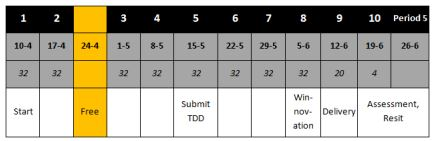
\includegraphics[scale=1.25]{images/schedule.JPG}
    \caption{Schedule}\label{fig:fuzzy-distance}
\end{figure}

Our sprints are two weeks long. On the first day of the sprint we will make our sprint planning. Every day we will be doing a daily scrum meeting. At the end of a sprint we will do a retrospective.


\newpage

\section{Presence}
In this chapter we will give insight into the members of the team, the team's presence at school and how we will handle absence.

\subsection{Team}
The team consists of the following members:
\begin{itemize}
  \item Sander Bouwman (S1080528)
  \item Stephan Schrijver (S1078783)
  \item Jeroen Vinke (S1078666)
  \item Robin Koning (S1078710)
  \item Mark van der Woude (S1081655)
\end{itemize}
\subsection{Presence}
The team is working on the project for 4 days a week. Which day we are not working on the project could differ per week. We handle absence by making up for the missed time in our own time. We are all adults and trust each other to keep up with the team.




\newpage

\section{Additional}
\blindtext

\newpage

\bibliography{bib/sources}
\newpage

\section{Appendix}
\begin{figure}[!htb]
    \centering
    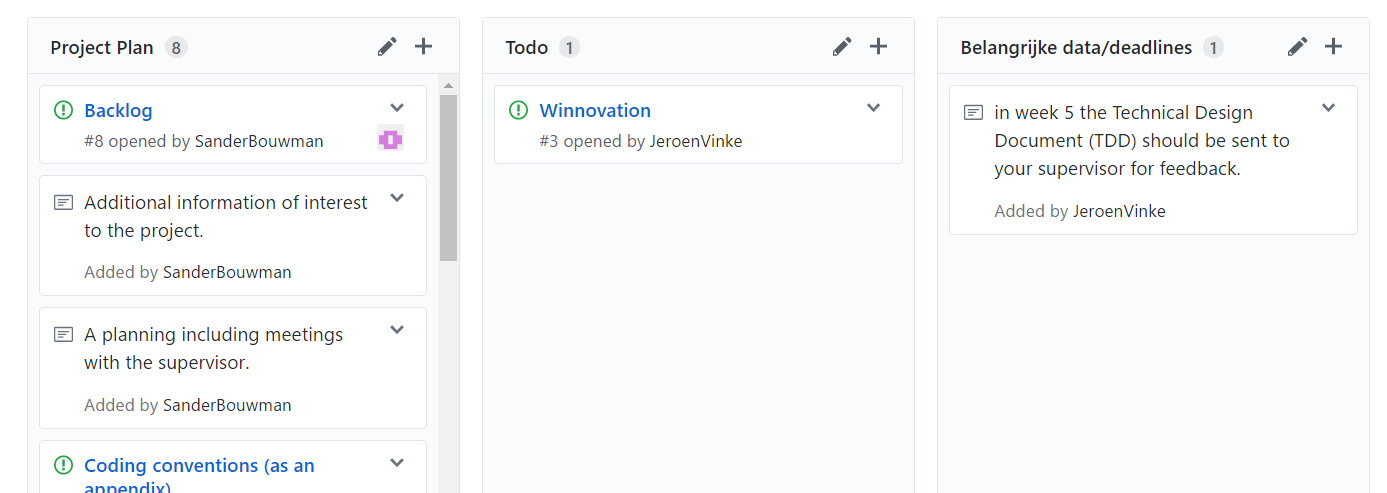
\includegraphics[angle=-90,origin=c,scale=0.75]
    {images/github-projects.PNG}
    \caption{GitHub project}\label{fig:githubproject}
\end{figure}

\end{document}

